\FloatBarrier
\paragraph{Unforced energy dissipation.}
We next test free relaxation on the fixed $K=8$ mesh, with $T=0.5$
and $\dt=1/16,1/32,1/64$. All physical parameters remain one.
Unlike the manufactured-solution test, the applied field and all
compensating sources are set to zero:
$\bs H_e=\bs f=\bs g=\bs r=0$.
We retain the homogeneous boundary traces described above.
The initial shapes are
\[
\bs u_0=C_u^{-1}\nabla B\times a,\qquad
\bs\omega_0=C_\omega^{-1}B b,\qquad
\bs m_0=C_m^{-1}S c.
\]
The initial velocity is projected onto the discrete solenoidal space;
angular velocity and magnetization are interpolated into their
respective spaces. The initial potential is recomputed with zero
boundary trace from
\[
(\nabla\varphi_h^0,\nabla\psi_h)
=-(\bs m_h^0,\nabla\psi_h)
\qquad\text{for all admissible }\psi_h,
\]
rather than prescribed from the manufactured magnetic potential.
The auxiliary variables satisfy their discrete projection relations.
Thus the internal magnetic field is not artificially suppressed,
and the subsequent solution is not constrained to follow the
manufactured temporal profile.

At every time level we integrate the discrete energy
\begin{equation}\label{eq:energy-test-observable}
E_h^n=\frac12\left(
\rho\|\bs u_h^n\|^2+
\rho\kappa\|\bs\omega_h^n\|^2+
\|\bs m_h^n\|^2+
\mu_0\|\nabla\varphi_h^n\|^2\right).
\end{equation}
The norms in \eqref{eq:energy-test-observable} are spatial $L^2$ norms.
Energy and dissipation are evaluated in the original finite-element
spaces using degree-12 quadrature, not from the visualization fields.
We also check the balance defect
\begin{equation}\label{eq:energy-test-first-balance}
R_h^n=E_h^n-E_h^{n-1}+\dt D_h^n+N_h^n,
\qquad
N_h^n=\tfrac12\|\mathcal X_h^n-\mathcal X_h^{n-1}\|_{\mathtt D}^2,
\end{equation}
where $D_h^n$ is the discrete viscous, spin, magnetic-diffusion,
and relaxation dissipation corresponding to $\mathtt A$.
In particular, the weak magnetic diffusion terms are evaluated as
$\sigma\|\bs k_h^n\|^2$ and
$\sigma\mu_0\|\vartheta_h^n\|^2$.
For both schemes, the reported balance diagnostic is
\[
\epsilon_{\rm bal}^n=
\frac{|R_h^n|}{\max\{E_h^n,E_h^{n-1},\dt D_h^n+N_h^n,
10^{-14}E_h^0\}},
\]
with the midpoint dissipation and $N_h^n=0$ used for the
second-order scheme.

All energy runs use 48 MPI processes with one thread each and the
same five-block solver settings as the convergence experiments.
The first-order runs require no nonlinear startup.
\Cref{fig:first-order-energy} shows monotone decay for all three
time steps. The initial discrete energy is approximately
$4.205865\times10^{-2}$; the final energy ratios and balance
diagnostics are given in \Cref{tab:first-order-energy}.
The largest balance diagnostic is $4.61\times10^{-14}$.
These results verify dissipation for the tested discretizations;
they do not constitute a pure temporal convergence study.

\begin{table}[htbp]
\centering
\caption{First-order unforced energy test: $K=8$, $T=0.5$.}
\label{tab:first-order-energy}
\small
\begin{tabular}{crr}
\toprule
$\dt$ & $E_h(T)/E_h(0)$ & $\max_n\epsilon_{\rm bal}^n$\\
\midrule
$1/16$ & $9.1847\times10^{-5}$ & $3.69\times10^{-14}$\\
$1/32$ & $3.1955\times10^{-5}$ & $2.22\times10^{-14}$\\
$1/64$ & $1.6247\times10^{-5}$ & $4.61\times10^{-14}$\\
\bottomrule
\end{tabular}
\end{table}

\begin{figure}[htbp]
\centering
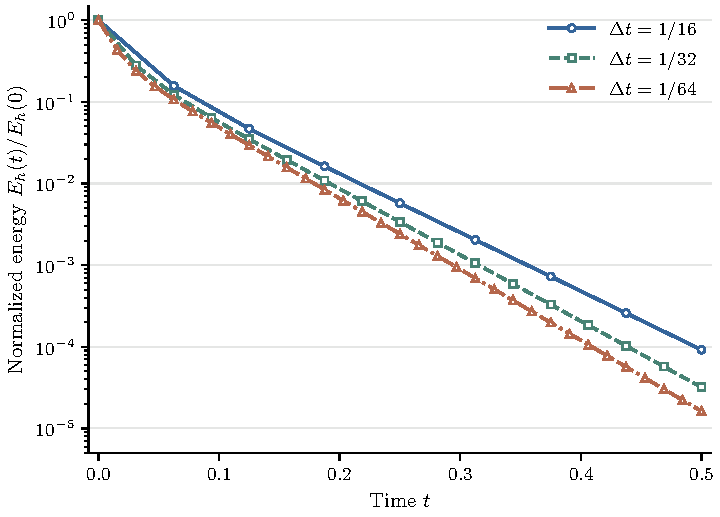
\includegraphics[width=0.70\textwidth]{figures/first_order_energy.pdf}
\caption{Normalized discrete energy for the first-order scheme in the
unforced relaxation test, $K=8$ and $T=0.5$.
The vertical axis is logarithmic. Symbols represent all computed time
levels; connecting lines are not fitted or smoothed curves.
The same discrete initial state is used for all three time steps.}
\label{fig:first-order-energy}
\end{figure}
\FloatBarrier
